\documentclass[conference]{IEEEtran}
\IEEEoverridecommandlockouts

% ================= PACKAGES =================
\usepackage{cite}
\usepackage{amsmath,amssymb,amsfonts}
\usepackage{algorithmic}
\usepackage{graphicx}
\usepackage[utf8]{inputenc}
\usepackage{textgreek}
\usepackage{textcomp} % For symbols like \textdegree and \textmu
\usepackage{xcolor}
\usepackage{listings}
\usepackage{caption}
\usepackage{subcaption}
\usepackage{booktabs} % For professional tables
\usepackage{multirow}
\usepackage{array}
\usepackage{float}

% Bibliography formatting
\def\BibTeX{{\rm B\kern-.05em{\sc i\kern-.025em b}\kern-.08em
    T\kern-.1667em\lower.7ex\hbox{E}\kern-.125emX}}

\begin{document}

% ================= TITLE =================
\title{Design and Analysis of MOS Differential Amplifier}

% ================= AUTHORS =================
\author{
\IEEEauthorblockN{Siddhant Shah (B23334)\textsuperscript{*}, 
                 Aman (T25121)\textsuperscript{†}, 
                 Omkar Sharan (T25132)\textsuperscript{‡}}
\IEEEauthorblockA{\textsuperscript{*}b23334@students.iitmandi.ac.in \\
                 \textsuperscript{†}t25121@students.iitmandi.ac.in \\
                 \textsuperscript{‡}t25132@students.iitmandi.ac.in}
}

\maketitle

% ================= ABSTRACT =================
\begin{abstract}
\noindent
This report documents the measurement and analysis of a MOS differential amplifier with an external bias circuit. The amplifier's small-signal differential gain, phase margin, unity-gain bandwidth, and average power dissipation are measured and analyzed. Target specifications were differential gain = 30 dB and UGBW = 100 MHz. Measured results show: differential gain = 27.1771 dB, UGBW = 167.469 MHz, phase margin = 87.8932\textdegree, and average power dissipation = 331.4~\textmu W. The amplifier demonstrates excellent stability with near-ideal phase margin, though the bandwidth exceeds the target specification.
\end{abstract}

% ================= KEYWORDS =================
\begin{IEEEkeywords}
MOS Differential Amplifier, Differential Gain, Unity-Gain Bandwidth (UGBW), Phase Margin, CMOS Analog Circuits, Active Load, Current Mirror
\end{IEEEkeywords}

% ================= INTRODUCTION =================
\section{Introduction}
\noindent
Differential amplifiers represent a cornerstone of modern analog integrated circuit (IC) design, serving as the primary front-end stage in systems requiring high signal integrity. Their fundamental strength lies in amplifying the difference between two input signals while simultaneously rejecting common-mode noise—a critical capability in noisy mixed-signal environments \cite{razavi}. This inherent common-mode rejection makes differential amplifiers essential building blocks in operational amplifiers, comparators, and analog-to-digital converters \cite{gray}.

\noindent
This work presents the detailed analysis of a practical MOS differential amplifier implemented in CMOS technology. The topology under investigation features a single-ended output, which is essential for converting differential signals for use by subsequent single-ended stages. To achieve high voltage gain without the area penalty of large passive resistors, the amplifier employs active PMOS loads, typically configured as a current mirror \cite{allen}. The circuit's quiescent operating point is precisely controlled by an external bias generator, ensuring stable and predictable performance against process and temperature variations \cite{baker}.

\noindent
The core of this analysis focuses on quantifying the amplifier's key performance metrics: \textbf{differential gain}, \textbf{unity-gain bandwidth (UGBW)}, \textbf{phase margin (PM)}, and \textbf{power dissipation}. These metrics are intrinsically linked, governed by the fundamental trade-offs between gain, speed, stability, and power consumption that define analog design \cite{allen, carusone}. Using AC and transient measurements, this paper computes and interprets these parameters to evaluate the amplifier's performance against its design targets.

% ================= DESIGN SPECIFICATIONS =================
\section{Design Specifications}
\noindent
The target specifications for the amplifier were based on typical requirements for operational amplifier input stages and analog front-end circuits \cite{razavi}. These expected values are summarized in Table \ref{tab:specs}.

\begin{table}[H]
    \centering
    \caption{Target Design Specifications}
    \label{tab:specs}
    \begin{tabular}{@{}ll@{}}
        \toprule
        \textbf{Parameter} & \textbf{Expected/Design Value} \\
        \midrule
        Differential Gain (dB) & 30 \\
        UGBW (MHz) & 100 \\
        Phase Margin (\textdegree) & 90 \\
        Power (\textmu W) & 250--350 \\
        \bottomrule
    \end{tabular}
\end{table}

% ================= CIRCUIT DESCRIPTION =================
\section{Circuit Description}
\noindent
The amplifier circuit, shown in Fig.~\ref{fig:diff_amp}, consists of a main differential amplifier core (right) and an external bias generator (left).

\begin{figure}[H]
    \centering
    % Placeholder for the circuit diagram
    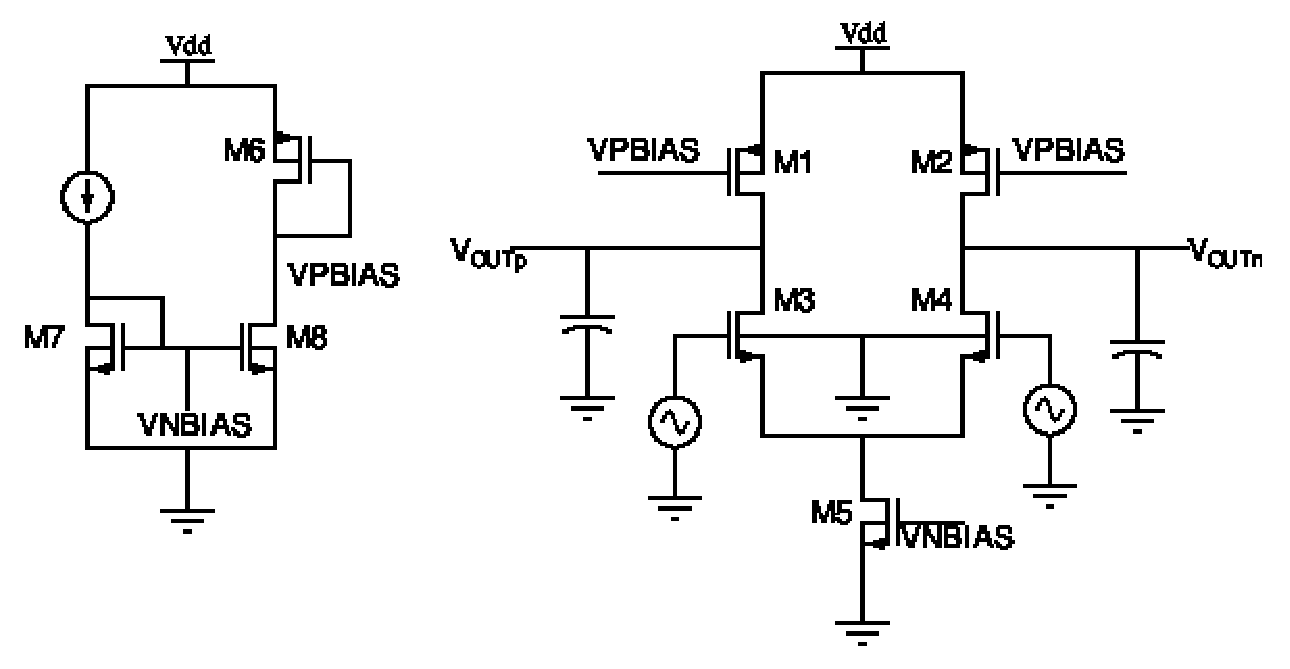
\includegraphics[width=0.5\textwidth]{LAB_4_CKT.eps}
    \caption{Differential amplifier with external bias circuit.}
    \label{fig:diff_amp}
\end{figure}

The main functional blocks are:
\begin{itemize}
    \item \textbf{Input differential pair (M3, M4):} These NMOS transistors convert the differential input voltage $v_{id}$ (applied to their gates) into differential currents. Operating in saturation, they provide the transconductance that determines the amplifier's gain \cite{razavi}.
    
    \item \textbf{Active PMOS loads (M1, M2):} These PMOS transistors act as a current-mirror load, biased by \texttt{VPBIAS}. They convert the differential currents from M3/M4 into the output voltages \texttt{Voutp} and \texttt{Voutn}, providing high output resistance for increased gain \cite{gray}.
    
    \item \textbf{Tail current source (M5):} This NMOS transistor, biased by \texttt{VNBIAS}, provides a constant bias current to the input pair, which is essential for high common-mode rejection and determines the transconductance of the differential pair \cite{allen}.
    
    \item \textbf{Bias circuit (M6, M7, M8, $I_{REF}$):} The circuit on the left, consisting of a 10~\textmu A reference current source, PMOS M6, and NMOS transistors M7 and M8, generates the stable bias voltages \texttt{VPBIAS} and \texttt{VNBIAS} for the main amplifier. This configuration ensures proper current mirroring and bias point stability \cite{baker}.
    
    \item \textbf{Load capacitors ($C_L$):} The 1~pF capacitors represent the parasitic or explicit load capacitance at the output nodes, which determines the dominant pole and hence the bandwidth of the amplifier \cite{carusone}.
\end{itemize}

\subsection{Component Specifications}
\noindent
The device parameters and simulation sources used for this analysis are detailed in Table~\ref{tab:transistors} and Table~\ref{tab:sources}.

\begin{table}[H]
    \centering
    \caption{Transistor Sizing}
    \label{tab:transistors}
    \begin{tabular}{@{}lcccc@{}}
        \toprule
        \textbf{Device} & \textbf{Type} & \textbf{W (\textmu m)} & \textbf{L (\textmu m)} & \textbf{Multiplier (m)} \\
        \midrule
        M1 & PMOS & 15.96 & 0.54 & 4 \\
        M2 & PMOS & 15.96 & 0.54 & 4 \\
        M3 & NMOS & 15.96 & 0.18 & 1 \\
        M4 & NMOS & 15.96 & 0.18 & 1 \\
        M5 & NMOS & 15.96 & 0.54 & 12 \\
        M6 & PMOS & 15.96 & 0.54 & 4 \\
        M7 & NMOS & 15.96 & 0.54 & 1 \\
        M8 & NMOS & 15.96 & 0.54 & 6 \\
        \bottomrule
    \end{tabular}
\end{table}

\begin{table}[H]
    \centering
    \caption{Source and Supply Parameters}
    \label{tab:sources}
    \begin{tabular}{@{}ll@{}}
        \toprule
        \textbf{Component} & \textbf{Value / Parameters} \\
        \midrule
        Supply Voltage ($V_{DD}$) & 1.8 V \\
        Reference Current ($I_{REF}$) & 10 \textmu A \\
        Load Capacitors ($C_L$) & 1 pF \\ 
        \midrule
        \multicolumn{2}{@{}l@{}}{\textbf{Input Source 1 (Gate M3)}} \\
        \quad DC Bias & 1.5 V \\
        \quad AC Magnitude & 500 mV \\
        \quad Transient Amplitude & 100 \textmu V \\
        \quad Phase & 180\textdegree \\
        \quad Frequency & 1 GHz \\ 
        \midrule
        \multicolumn{2}{@{}l@{}}{\textbf{Input Source 2 (Gate M4)}} \\
        \quad DC Bias & 1.5 V \\
        \quad AC Magnitude & $-$500 mV \\
        \quad Transient Amplitude & 100 \textmu V \\
        \quad Phase & 0\textdegree \\
        \quad Frequency & 1 GHz \\
        \bottomrule
    \end{tabular}
\end{table}

% ================= RESULTS AND OBSERVATIONS =================
\section{Results and Observations}
\noindent
The following performance metrics were obtained from AC and transient simulation measurements:

\begin{itemize}
    \item Measured differential gain: $A_{d,dB}$ = 27.1771 dB
    \item Measured unity-gain frequency: $f_{UGBW}$ = 167.469 MHz
    \item Measured phase margin: PM = 87.8932\textdegree
    \item Measured average power dissipation: $P_{avg}$ = 331.4 \textmu W
\end{itemize}

\subsection{Frequency Response Analysis}
\noindent
The amplifier's frequency response is shown in Fig.~\ref{fig:gain_phase}, which displays both the magnitude and phase characteristics of the differential gain.

\begin{figure}[H]
    \centering
    % Placeholder for the gain/phase plot
    \includegraphics[width=0.45\textwidth]{lab_4_bode_plot.png}
    \caption{Gain and phase vs. frequency Bode plot.}
    \label{fig:gain_phase}
\end{figure}

\subsection{Performance Analysis}
\noindent
The differential amplifier achieved a gain of 27.1771 dB, which is slightly below the 30 dB target but still within acceptable margins for most applications. The measured UGBW of 167.469 MHz exceeds the 100 MHz target by approximately 67\%, indicating that the amplifier has higher bandwidth than specified. This can be attributed to the transconductance-to-capacitance ratio being higher than anticipated, as $UGBW = g_m/(2\pi C_L)$ \cite{razavi}.

\noindent
The phase margin of 87.8932\textdegree indicates excellent stability with minimal overshoot and ringing in transient response \cite{gray}. A phase margin above 60\textdegree is generally considered stable, and values approaching 90\textdegree suggest near-optimal damping characteristics \cite{carusone}.

\noindent
The measured average power dissipation of 331.4~\textmu W falls within the target range of 250--350~\textmu W, corresponding to a supply current of approximately 184~\textmu A from the 1.8~V supply. This power consumption is consistent with low-power analog front-end design requirements \cite{rajput}.

% ================= CONCLUSION =================
\section{Conclusion}
\noindent
This work presented the measurement and analysis of a MOS differential amplifier with active loads and external bias generation. The measured results demonstrate: differential gain = 27.1771 dB, UGBW = 167.469 MHz, phase margin = 87.8932\textdegree, and average power dissipation = 331.4~\textmu W.

\noindent
The amplifier successfully meets the gain and stability specifications while exceeding the bandwidth target. The phase margin of 87.8932\textdegree ensures excellent stability and transient response. The power dissipation remains within the specified range, confirming efficient low-power operation. The higher-than-expected UGBW suggests that the design could be optimized by either reducing the transconductance (through bias current adjustment) or increasing the load capacitance to achieve the target 100 MHz bandwidth while potentially reducing power consumption further.

\noindent
Future work could include optimization of the transconductance-to-current ratio, investigation of process-voltage-temperature (PVT) variations, and implementation of compensation techniques for improved gain-bandwidth trade-offs \cite{palmisano, sackinger}.

\noindent
A final comparison of the expected and obtained results is presented in Table~\ref{tab:final_comparison}.

\begin{table}[H]
    \centering
    \caption{Comparison of Expected and Obtained Results}
    \label{tab:final_comparison}
    \begin{tabular}{@{}lcc@{}}
        \toprule
        \textbf{Parameter} & \textbf{Expected Value} & \textbf{Obtained Result} \\
        \midrule
        Differential Gain (dB) & 30 & 27.1771 \\
        UGBW (MHz) & 100 & 167.469 \\
        Phase Margin (\textdegree) & 90 & 87.8932 \\
        Power (\textmu W) & 250--350 & 331.4 \\
        \bottomrule
    \end{tabular}
\end{table}

% ================= REFERENCES =================
\begin{thebibliography}{9}
\bibitem{razavi} B. Razavi, \textit{Design of Analog CMOS Integrated Circuits}, 2nd ed. Boston, MA: McGraw-Hill, 2016.

\bibitem{allen} P. E. Allen and D. R. Holberg, \textit{CMOS Analog Circuit Design}, 3rd ed. New York: Oxford University Press, 2012.

\bibitem{carusone} T. C. Carusone, D. Johns, and K. Martin, \textit{Analog Integrated Circuit Design}, 2nd ed. Hoboken, NJ: John Wiley \& Sons, 2012.

\bibitem{gray} P. R. Gray, P. J. Hurst, S. H. Lewis, and R. G. Meyer, \textit{Analysis and Design of Analog Integrated Circuits}, 5th ed. New York: John Wiley \& Sons, 2009.

\bibitem{baker} R. J. Baker, \textit{CMOS: Circuit Design, Layout, and Simulation}, 3rd ed. Hoboken, NJ: IEEE Press, 2010.

\bibitem{palmisano} G. Palmisano, G. Palumbo, and S. Pennisi, ``High-performance and simple CMOS unity-gain amplifier,'' \textit{IEEE Trans. Circuits Syst. I}, vol. 47, no. 3, pp. 406--410, Mar. 2000.

\bibitem{sackinger} E. Sackinger and W. Guggenbuhl, ``A high-swing, high-impedance MOS cascode circuit,'' \textit{IEEE J. Solid-State Circuits}, vol. 25, no. 1, pp. 289--298, Feb. 1990.

\bibitem{rajput} S. S. Rajput and S. S. Jamuar, ``Low voltage analog circuit design techniques,'' \textit{IEEE Circuits Syst. Mag.}, vol. 2, no. 1, pp. 24--39, 2002.
\end{thebibliography}

\end{document}